\documentclass[a4paper]{article}

%% Language and font encodings
\usepackage[spanish]{babel}
\usepackage[utf8x]{inputenc}
\usepackage[T1]{fontenc}
\usepackage{listings}
\spanishdecimal{.}


%% Sets page size and margins
\usepackage[a4paper,top=3cm,bottom=2cm,left=3cm,right=3cm,marginparwidth=1.75cm]{geometry}

%% Useful packages
\usepackage{amsmath}
\usepackage{graphicx}
\usepackage[colorinlistoftodos]{todonotes}
\usepackage[colorlinks=true, allcolors=blue]{hyperref}

\title{Práctica 9: interacciones entre partículas}
\begin{document}
\maketitle

\section{Introducci\'on}
Tenemos un grupo de partículas que habitan en un mismo espacio, lo que se ejemplifica en esta práctica, será un poco la interacción que poseen una con otra, la distancia que ellas recorren a lo largo del tiempo y el modo de desplazarse. Toda la primera sección de la práctica se hará referencia tanto la la tarea como al reto uno, los cuales consisten en asignarle un cierto peso a cada una de las partículas, así como observar el cambio de velocidad con la que se mueve y delimitar la relación que posee su masa con la velocidad. Par el reto uno lo que se desea es que la representación gráfica de las partículas dependa ahora de los tamaños de la masa, es decir que posean un radio de dimensión proporcional al de su peso. La partícula de inicio posee una coordenada en cada eje \texttt{x} y \texttt{y}, así como una carga, como lo es en la vida ordinaria, las cargas iguales se repelen y las opuestas se atraen, así mismo se les fue asignado un peso.

\section{Par\'ametros de trabajo}
Las pruebas se corrieron en una iMac con procesador 3.1 Ghz, Intel Core i7 con 16 GB de memoria y 1600 Mhz y con ocho núcleos. Se contemplarán los requerimientos del reto uno, así la variable \textit{n} representa la cantidad total de partículas, de esta forma existirán $50$. La prueba fue corrida con panorama de tiempo de cien movimientos, es decir las partículas se desplazaron y actualizaron su posición cien veces.

\section{Modificaciones del código}
Para poder rescatar los cambios de posición y medir la distancia recorrida para la tarea original fue necesario modificar la forma en la que actualizaba las variables de posición. Así mismo se incluyó una columna más al \textit{data.frame} original, en el cual fueran asignados los pesos de la partícula en proporción a su carga original.

\begin{lstlisting}[frame=single]
c=rnorm(n)
m <- (floor(abs(c)*50) + 1)
p <- data.frame(x = rnorm(n), y=rnorm(n),c, m)
tiemx <- c()
tiemy <- c()
\end{lstlisting}

Así mismo se crearon los vectores \texttt{tiemx} y \texttt{tiemy} con el fin de utilizarlos más adelante para salvar las posiciones de las partículas, los cuales son empleados en la paralelización como se muestra. De igual forma para calcular las distancias de los movimientos se incluye la variable distancia, la cual por el modo en el que están guardados los datos te ayuda para el cálculo. Se llegó a la conclusión que no era necesario hacer el ciclo de distancia como una función propiamente ni paralelizarlo, ya que el programa tardaba más tiempo en ejecutarse. Así mismo se muestra la forma que afecta al \texttt{delta} el peso de la partícula.

\begin{lstlisting}[frame=single]
for (iter in 1:tmax) {
...
 p$x <- foreach(i = 1:n, .combine=c) %dopar% max(min(p[i,]$x + 
 (delta/p[i,]$m) * f[c(TRUE, FALSE)][i], 1), 0)
 tiemx <- c(tiemx,p$x)
 p$y <- foreach(i = 1:n, .combine=c) %dopar% max(min(p[i,]$y + 
 (delta/p[i,]$m) * f[c(FALSE, TRUE)][i], 1), 0)
 tiemy <- c(tiemy,p$y)
...
}
distancia <- c()
for(i in 1:(n*(tmax))){
distancia <- c(distancia, ((tiemx[i]-tiemx[i+50])^2 + 
(tiemy[i]-tiemy[i+50])^2)^(1/2))
}
\end{lstlisting}
Para generar el gráfico adecuado de los datos por tamaño de partícula como lo pide el reto uno fue necesario crear otro \texttt{data.frame} con el fin de generar una gráfica tipo \texttt{boxplot} que representara los tiempos respecto a la masa, como se muestra en la figura \ref{fig:totaloriginal} así como grabar los datos en un archivo tipo \texttt{.csv} con el fin de no perder los datos y poder usarlos en futuro.

\begin{lstlisting}[frame=single]
total <- data.frame(iteraciones,distancia,masa)
total$masa <- as.factor(total$masa)
library('ggplot2')
png(paste("totalR.png", sep=""), width=700, height=700)
ggplot(data=total,aes(x=masa,y=distancia,fill=iteraciones))+
geom_boxplot()#stat_summary(fun.y=mean,geom="smooth",
aes(group=Tipo,col=Tipo))
graphics.off()

write.csv(total,file="TotalReto.csv")
\end{lstlisting}
La última modificación que se realizó fue la generación de los grafos respetando el tamaño de la partícula es decir respecto a la masa asignada, a continuación solo se muestra la instrucción para generarla de una sola posición de partículas, así como la figura \ref{fig:p9i} muestra los diferentes radios de las partículas y de forma similar son las instrucciones para el resto de las imágenes.

\begin{lstlisting}[frame=single]
  png("p9radios.png")
  grafica <- ggplot(p, aes(x=p$x, y=p$y))
  grafica+geom_point(aes(size= p$m,col=colores[p$g+6]))+ 
  xlab("x")+ ylab("y") + 
  labs(color= "carga", size="masa")+
  scale_color_manual(labels=seq(5,-5,-1),values=colores)+
  guides(col= guide_legend(override.aes = list(size=3, stroke=1.5))) +
  scale_size_continuous(breaks=seq(0,0.1,0.01),labels=seq(0,0.1,0.01))
  graphics.off()
\end{lstlisting}

\begin{figure}[h]
\centering
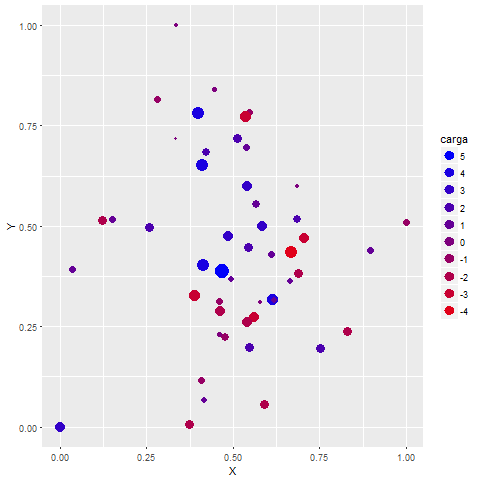
\includegraphics[width=0.7\linewidth]{p9i}
\caption{Partículas con masa y radio.}
\label{fig:p9i}
\end{figure}


\section{Resultados}
La figura \ref*{fig:totaloriginal} nos muestra la práctica original y es un poco de esperar la relación que muestran las distancias respecto a las cargas, mientras es más fuerte la carga que posee la partícula es más el desplazamineto que se realiza en ella.

\begin{figure}[h!]
\centering
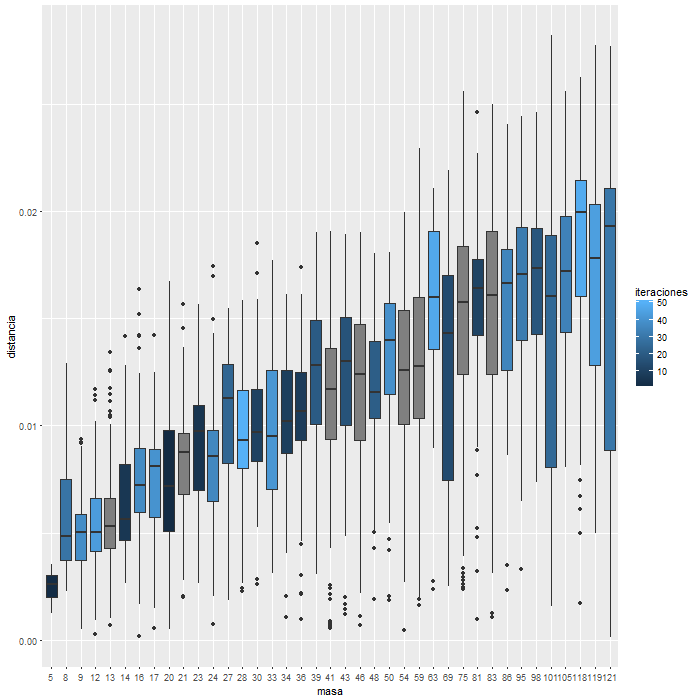
\includegraphics[width=0.7\linewidth]{totaloriginal}
\caption{Distancias recorridas con respecto a la carga considerando que todas las masas son iguales.}
\label{fig:totaloriginal}
\end{figure}

En cambio observemos la figura \ref{fig:totalR}, en ella podemos observar de igual forma el tiempo pero ahora respecto a la cantidad de masa, la cual como ya mencionamos esta relacionada de cierta forma a la cantidad de carga proporcionada a ella. En la imagen podemos observar que mientras mayor es la masa del objeto, menor es su movimiento, en las partículas pequeñas los movimientos son sumamente grandes y conformo aumenta la masa se puede observar que los movimientos son mucho más pequeños.

\begin{figure}[h!]
\centering
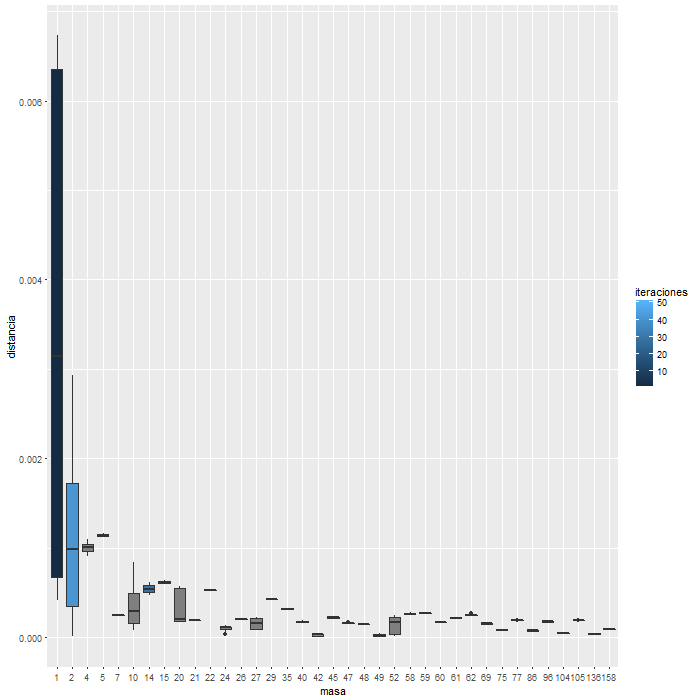
\includegraphics[width=0.7\linewidth]{total}
\caption{Distancias recorridas respecto a su cantidad de masa.}
\label{fig:totalR}
\end{figure}

\section{Comentarios}
Se incluyen tres GIF, el primero de ellos, \href{https://github.com/ValeryGomez/SimulacionSistemas/blob/master/P9/MasaIgual.gif}{MasaIgual} muestra el movimiento original de las partículas sin ninguna masa que los haga ir más rápido o menos. El segundo GIF que se incluye \href{https://github.com/ValeryGomez/SimulacionSistemas/blob/master/P9/Peso.gif}{Peso} se muestran las partículas con sus respectivos pesos pero aún sin visualización de su radio. Y el último GIF \href{https://github.com/ValeryGomez/SimulacionSistemas/blob/master/P9/Radios.gif}{Radio} las muestra ya con su respectivo radio, es decir en proporción al tamaño de su masa y su mismo movimiento.

\end{document}